\begin{problem}
Найти и построить область определения функции
\[ z = \ln(y - \ln x). \]
\end{problem}

\begin{solution}
  Функция $\ln(u)$ определена тогда и только тогда, когда её   аргумент $u > 0$. 
  
  В нашем случае:
  \[y - \ln x > 0 \quad \Rightarrow \quad y > \ln x. \]
  и:
  \[x > 0 \quad \]
  Тогда D:
  \[D = \{(x, y) \in {R}^2 \mid x > 0,\ y > \ln x\}\]

Границы области:
\begin{itemize}
    \item $y = \ln x$
    \item $x = 0$
\end{itemize}

Проверим некоторые точки:
\begin{itemize}
    \item Точка $(1, 0)$: $\ln 1 = 0$; $y > 0$
    \item Точка $(e, 1)$: $\ln e = 1$; $y > 1$
\end{itemize}

\vspace{20pt}

\textbf{График области определения:}

\begin{center}
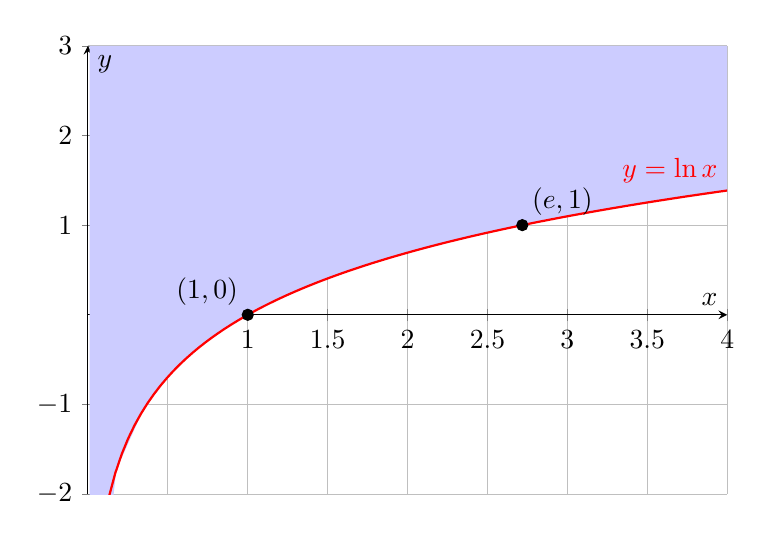
\begin{tikzpicture}
\begin{axis}[
    width=0.8\textwidth,
    height=0.6\textwidth,
    xmin=0, xmax=4,
    ymin=-2, ymax=3,
    axis lines=center,
    xlabel={$x$},
    ylabel={$y$},
    domain=0.01:4,
    samples=100,
    grid=major
]

\fill[blue!20] (0.01,-2) -- plot [domain=0.01:4] (\x,{ln(\x)}) -- (4,3) -- (0.01,3) -- cycle;

\addplot[red, thick] {ln(x)};
\node[red, left] at (axis cs:4,{ln(5)}) {$y = \ln x$};

\addplot[only marks, mark=*, mark size=2pt] coordinates {
    (1,0)
    (2.718,1)
};
\node[above left] at (axis cs:1,0) {$(1,0)$};
\node[above right] at (axis cs:2.718,1) {$(e,1)$};

\end{axis}
\end{tikzpicture}
\end{center}
\end{solution}